\section{Submodular}

\begin{frame}{Sensor placement}{Maximum coverage}
\begin{figure}
	\centering
	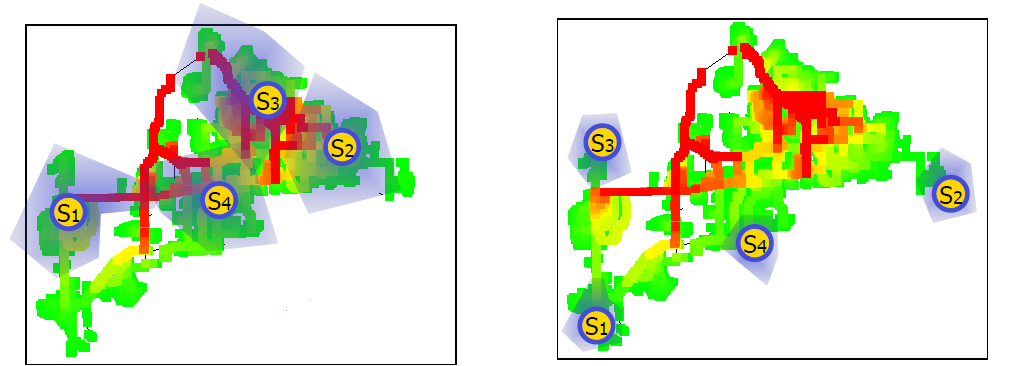
\includegraphics[width = \textwidth]{./figure/maximum_coverage}
\end{figure}
\begin{equation}
\nonumber
f( s_{1} , s_{2} , s_{3} , s_{4} ) \neq f( s_{1} ) + f( s_{2} ) + f( s_{3} ) + f( s_{4} )
\end{equation}	
\end{frame}

\begin{frame}{Sensor placement}{MAP inference}
\begin{figure}
	\centering
	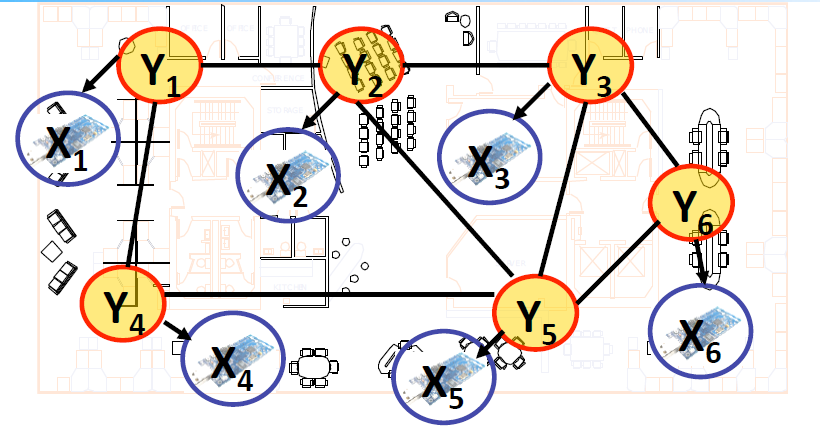
\includegraphics[width = .7 \textwidth]{./figure/map_inference}
\end{figure}
\begin{equation}
\nonumber
\log P( y \mid x_{1} , x_{2} , \cdots , x_{6} ) \neq \log P( y \mid x_{1} ) + \log P( y \mid x_{2} ) + \cdots + \log f( y \mid x_{6} )
\end{equation}		
\end{frame}

\begin{frame}{Submodularity}{Definition}
\begin{block}{Definition}
Let $ N $ be a finite ground set and $ f : 2^{N} \rightarrow R $. Then $ f $ is \textbf{submodular} if $ \forall A, B \subseteq N,
f(A) + f(B) \leq f(A \cup B) + f(A \cap B). $
\end{block}
\begin{itemize}
\item diminishing returns
\item equivalence : $ f(x \cup S) \leq f(x) + f(S) $
\end{itemize}
\end{frame}

\begin{frame}{Submodular+Supmodular+Modular}{Relationship}
\begin{block}{Supmodular}
$ - f(x) $ is submodular $ \Rightarrow $ $ f(x) $ is supmodular.
\end{block}
\begin{block}{Modular}
$ f(x) $ is both submodular and supmodular, $ f(x) $ is modular.
\begin{equation}
\nonumber
f( \mathbf{X} ) = \sum_{ x_{i} \in \mathbf{X} } f(x_{i})
\end{equation}
\end{block}
\end{frame}

\begin{frame}{Submodular}{Performance guarantee}
\begin{block}{Theorem (Nemhauser 1978)~\cite{nemhauser1978}}
Suppose $ f $ is monotonic and submodular. 
Then greedy algorithm gives constant factor approximation.
\begin{equation}
\nonumber
f(S_{greedy}) \geq (1 - \frac{1}{e}) f(S^{*})
\end{equation}	
\end{block}
\begin{itemize}
\item Provable near-optimal
\item Efficiency
\end{itemize}
\end{frame}